\begin{figure}[h]
    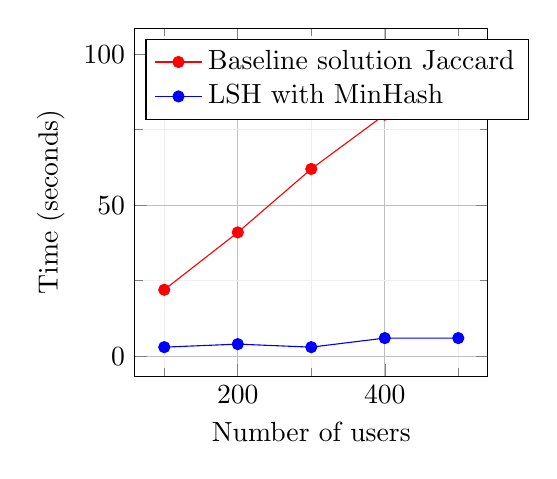
\begin{tikzpicture}
    \begin{axis}[
        xlabel=Number of users,
        ylabel=Time (seconds),
        height=6cm,
        width = 0.5*\textwidth,
        grid = both,
        minor tick num = 1,
        major grid style = {lightgray},
        minor grid style = {lightgray!25},
        legend cell align = {left},
        legend pos = north west
    ]
    
    % Add values and attributes for the first plot
    \addplot[color=red,mark=*] coordinates {
    	(100, 22)
    	(200, 41)
    	(300, 62)
    	(400, 80)
    	(500, 99)
    };
    
    % Add values and attributes for the second plot
    \addplot[color=blue,mark=*] coordinates {
    	(100, 3)
    	(200, 4)
    	(300, 3)
    	(400, 6)
    	(500, 6)
    };
    
    \legend{Baseline solution Jaccard,LSH with MinHash}
    \end{axis}
    \end{tikzpicture}
    \caption{\normalfont Time performance of the Naive algorithm compared with LSH using MinHash – Variable number of users}
    \label{fig:lsh_minhash_users}
\end{figure}
